
\documentclass[tikz,convert={convertexe={magick.exe}}]{standalone}

\begin{document}
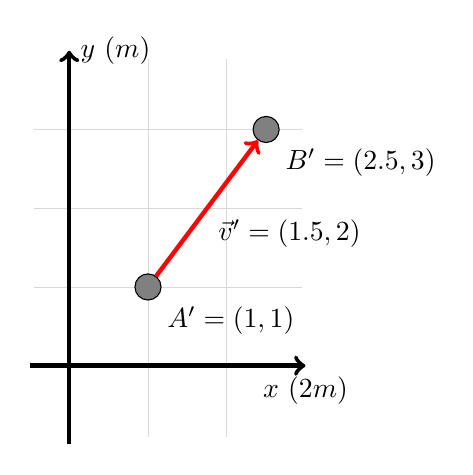
\begin{tikzpicture}[x=.5cm]
\draw[help lines, color=gray!30] (-.9,-.9) grid (5.9,3.9);
\draw[->, ultra thick] (-1,0)--(6,0) node[below]{$x$ ($2m$)};
\draw[->, ultra thick] (0,-1)--(0,4) node[right]{$y$ ($m$)};

\node (A) at (2,1) [circle, draw, fill=gray, label=below right:{$A' = (1,1)$}] {};
\node (B) at (5,3) [circle, draw, fill=gray, label=below right:{$B' = (2.5,3)$}] {};

\draw[->, ultra thick, red] (A) -- (B)
	node[midway, below right, black]{$\vec v' = (1.5,2)$};

\end{tikzpicture}
\end{document}